\section{Progettazione in frequenza per un sistema del secondo ordine}
	\label{app:sistemaSecondoordine}
	
	Una funzione di trasferimento del secondo ordine, può essere scritta in maniera del tutto generale come
	
	\begin{equation}
		H(s)=\frac{\omega_n^2}{s^2 + 2\xi \omega_ns + \omega_n^2}
		\label{eq:secondoOrdine}
	\end{equation}
	
	\noindent dove il parametro $\xi$ è il \textit{coefficiente si smorzamento} e $\omega_n$ è la \textit{pulsazione naturale non smorzata}. I poli di tale funzione di trasferimento sono una coppia complessa coniugata e si trovano ad una distanza dall'origine pari a $\omega_n$ e a un angolo $\theta=\arcsin\xi$. Una specifica naturale per le prestazione del sistema in termini di risposta in frequenza è la \textit{larghezza di banda}, definita come la frequenza massima alla quale il  sistema segue un ingresso sinusoidale in modo soddisfacente. Altro parametro importante è il valore massimo del modulo della  risposta in frequenza, denominato come picco di risonanza $S$. La larghezza di banda è una misura della prontezza di risposta e come tale corrisponde ad altri parametri, quali il tempo di salita e il tempo al picco nel dominio del tempo.
	
	\subsection{Sovraelongazione e tempo al picco}
		\label{subapp:sovraelongazionePicco}
		
		La massima sovraelongazione corrisponde al punto dove la derivata della risposta in frequenza del modulo si annulla. L'andamento nel tempo della risposta al gradino $H(s)/s$ si ottiene grazie alla trasformata di Laplace inversa
		
		\begin{equation}
			y(t) = 1 - e^{-\sigma t} \Big( \cos\omega_dt + \frac{\sigma}{\omega_d}\sin\omega_dt   \Big)
			\label{eq:rispostaGradino}
		\end{equation}  
		
		\noindent dove $\omega_d=\sqrt{1-\xi^2}$ e $\sigma=\xi\omega_n$. Utilizzando delle identità geometriche è possibile riscrivere l'equazione \ref{eq:rispostaGradino} in maniera più compatta
		
		\begin{equation}
			y(t) = 1-e^{-\sigma t}\sqrt{1 + \frac{\sigma^2}{\omega_d^2}}\cos(\omega_dt + \beta)
			\label{er:rispostaGradinoRiscritta}
		\end{equation}
		
		\noindent con $\beta=\arctan(\frac{\sigma}{\omega_d})$. Resta quindi da calcolare la sua derivata e porla pari a zero.
		
		\begin{align*}
			\dot{y}(t) &= \sigma e^{-\sigma t}\Big( \cos\omega_dt + \frac{\sigma}{\omega_d}\sin\omega_dt\Big) - e^{-\sigma t}(-\omega_d\sin\omega_d t + \sigma\cos\omega_d  t)=0 \\
			&= e^{-\sigma t}\Big( \frac{\sigma^2}{\omega_d}\sin\omega_dt +\omega_d\sin\omega_dt \Big)=0
		\end{align*}
		
		\noindent Questo si verifica quando $\sin\omega_dt=0$, dunque il tempo al picco $t_p$ risulta
		
		\begin{equation}
			t_p=\frac{\pi}{\omega_d}
			\label{eq:tempoPicco}
		\end{equation}
		
		\noindent Sostituendo \ref{eq:tempoPicco} dentro l'espressione di $y(t)$ si ottiene allora
		
		\begin{equation*}
			t(t_p)=1+S=1-e^{-\frac{\sigma\pi}{\omega_d}}\Big(\cos\pi+\frac{\sigma}{\omega_d}\sin\pi\Big)=1+e^{-\frac{\sigma\pi
			}{\omega_d}}
		\end{equation*}
		
		
		\begin{SCfigure}[\sidecaptionrelwidth][h!]
			\centering
			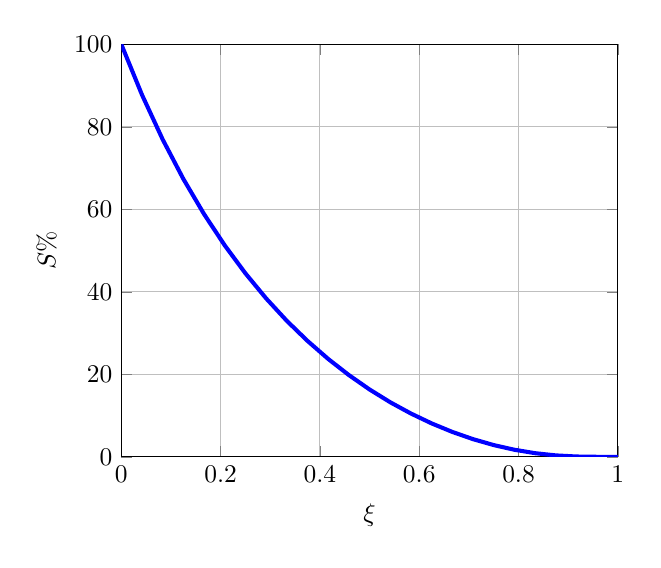
\begin{tikzpicture}[scale=0.92]				
				\begin{axis}[grid=both, xlabel=\phantom{$m_{\phi}^G$} $\xi$ \phantom{$m_{\phi}^G$}, ylabel=$S\singleSpacing \%$,enlargelimits=false]
			    	\addplot[domain=0:1, blue, ultra thick] {100*e^((-3.14*x)/(1-x^2)^(1/2)};
				\end{axis}	
			\end{tikzpicture}
			\caption{Relazione tra massima sovraelongazione $S$ e coefficiente di smorzamento $\xi$. \newline\newline\newline\newline\newline\newline\newline\newline\newline\newline\newline\newline}
			\label{fig:Sxi}		
		\end{SCfigure}
		
		\noindent Si ha dunque la seguente relazione, che lega la massima sovraelongazione al parametro $\xi$, a qui corrisponde il grafico di figura \ref{fig:Sxi}.
		
		\begin{empheq}[box=%
		\fbox]{equation}
			S = e^{-\frac{\pi\xi}{\sqrt{1-\xi^2}}}, \trippleSpacing 0 \le \xi < 1
			\label{eq:Sxi}
		\end{empheq}
		
		
		
	\subsection{Sovraelongazione e margine di fase}		
		\label{subapp:SovraelongazioneMargineFase}	
		
		Tenendo sempre in considerazione la funzione di trasferimento di un sistema del secondo ordine, descritta nell'equazione \ref{eq:secondoOrdine}, è possibile mostrare che la relazione tra il margine di fase $m^G_{\phi}$ e il coefficiente di smorzamento $\xi$ è
		
		\begin{equation}
			m^G_{\phi}=\arctan\Biggl[ \frac{2\xi}{\sqrt{\sqrt{1+4\xi^4}-2\xi^2}}  \Biggr]
			\label{eq:xiMG}
		\end{equation} 
		
		\noindent A questo punto è sufficiente invertire l'equazione \ref{eq:xiMG} e esplicitare la massima sovraelongazione $S$ in funzione del margine di fase $m^G_{\phi}$ utilizzando il risultato ottenuto prima, nella formula \ref{eq:Sxi}, ottenendo quindi il seguente risultato, qui proposto solo in via grafica.
		
		\begin{SCfigure}[\sidecaptionrelwidth][h!]
			\centering
			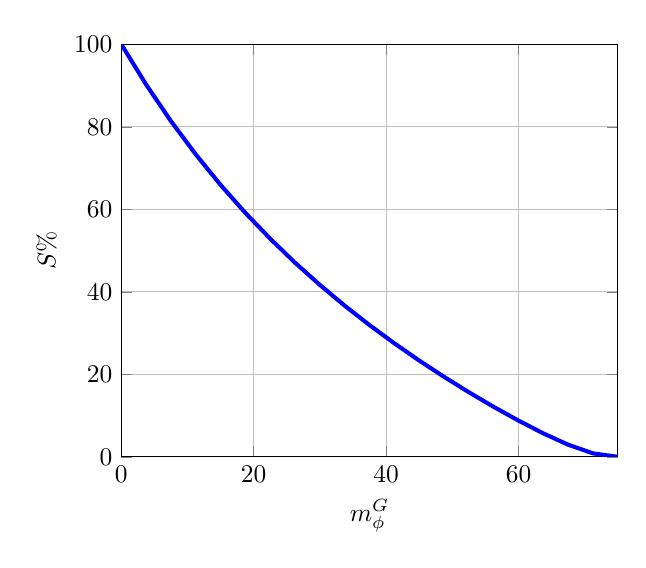
\begin{tikzpicture}[scale=0.92]
				\begin{axis}[grid=both, xlabel=$m_{\phi}^G$, ylabel=$S\singleSpacing \%$,enlargelimits=false]
			    	\addplot[domain=0:90, blue, ultra thick] {100*e^((-3.14*(tan(x)/(16*(tan(x))^2+16)^(1/4)))/((1-((tan(x)/(16*(tan(x))^2+16)^(1/4)))^2)^(1/2)))};
				\end{axis}
				
			\end{tikzpicture}
			\caption{Relazione tra massima sovraelongazione $S$ e margine di fase $m_{\phi}$.\newline\newline\newline\newline\newline\newline\newline\newline\newline\newline\newline\newline}
			\label{fig:mS}
		\end{SCfigure}		 
		